%\section{Results with additional differential observables with full Run 2 asimov datasets}
%Additional decay  observables include $\Phi$, $\Phi_{1}$, $\mathrm{m}(\mathrm{Z}_{1})$, $\mathrm{m}(\mathrm{Z}_{2})$, $|\cos \theta^{*}|$, $|\cos \theta_{1}|$, $|\cos \theta_{2}|$, number of jets (within $|\eta|<4.7$) and $\pt$ of leading jet (within $|\eta|<4.7$) which are studied in $\Hllll$ using full Run 2 toy data and compared with the theoretical predictions.
\subsection{Effective Field Theory interpretations}
To be updated.
%Differential measurements are extended upto higher dimension upto 2. Several 2D combination are aimed to be measured e.g. $\mathrm{m}(\mathrm{Z}_{1})$ vs $\mathrm{m}(\mathrm{Z}_{2})$ and so forth.
%To be updated further.
%Additional decay  observables include $\Phi$, $\Phi_{1}$, $\mathrm{m}(\mathrm{Z}_{1})$, $\mathrm{m}(\mathrm{Z}_{2})$, $|\cos \theta^{*}|$, $|\cos \theta_{1}|$ and $|\cos \theta_{2}|$  which are studied in $\Hllll$ using full Run 2 toy data and compared with the theoretical predictions.
%\par In each plot shown below, systematic uncertainty is indicated by red bars and black bars show total statistical and the systematic uncertainties, combined in quadrature. The blue and brown colors show the theoretical predictions. 
%          The acceptances and the theoretical uncertainties in differential bins are computed using {\sc powheg}. Sub-dominant production contribuu
%tions XH $=$ VBF $+$ VH $+$ $\ttH$ are shown in green separately. The systematic uncertainties correspond to the generators accuracy are also taken in to account for differential predictions. The fraction of $4\mu$, $4e$ and $2e2\mu$ in each differential bin is allowed to float in fit.
%\begin{figure}[!h!tb]
%  \begin{center}
%
%	  \subfigure[$\Phi$]{
%      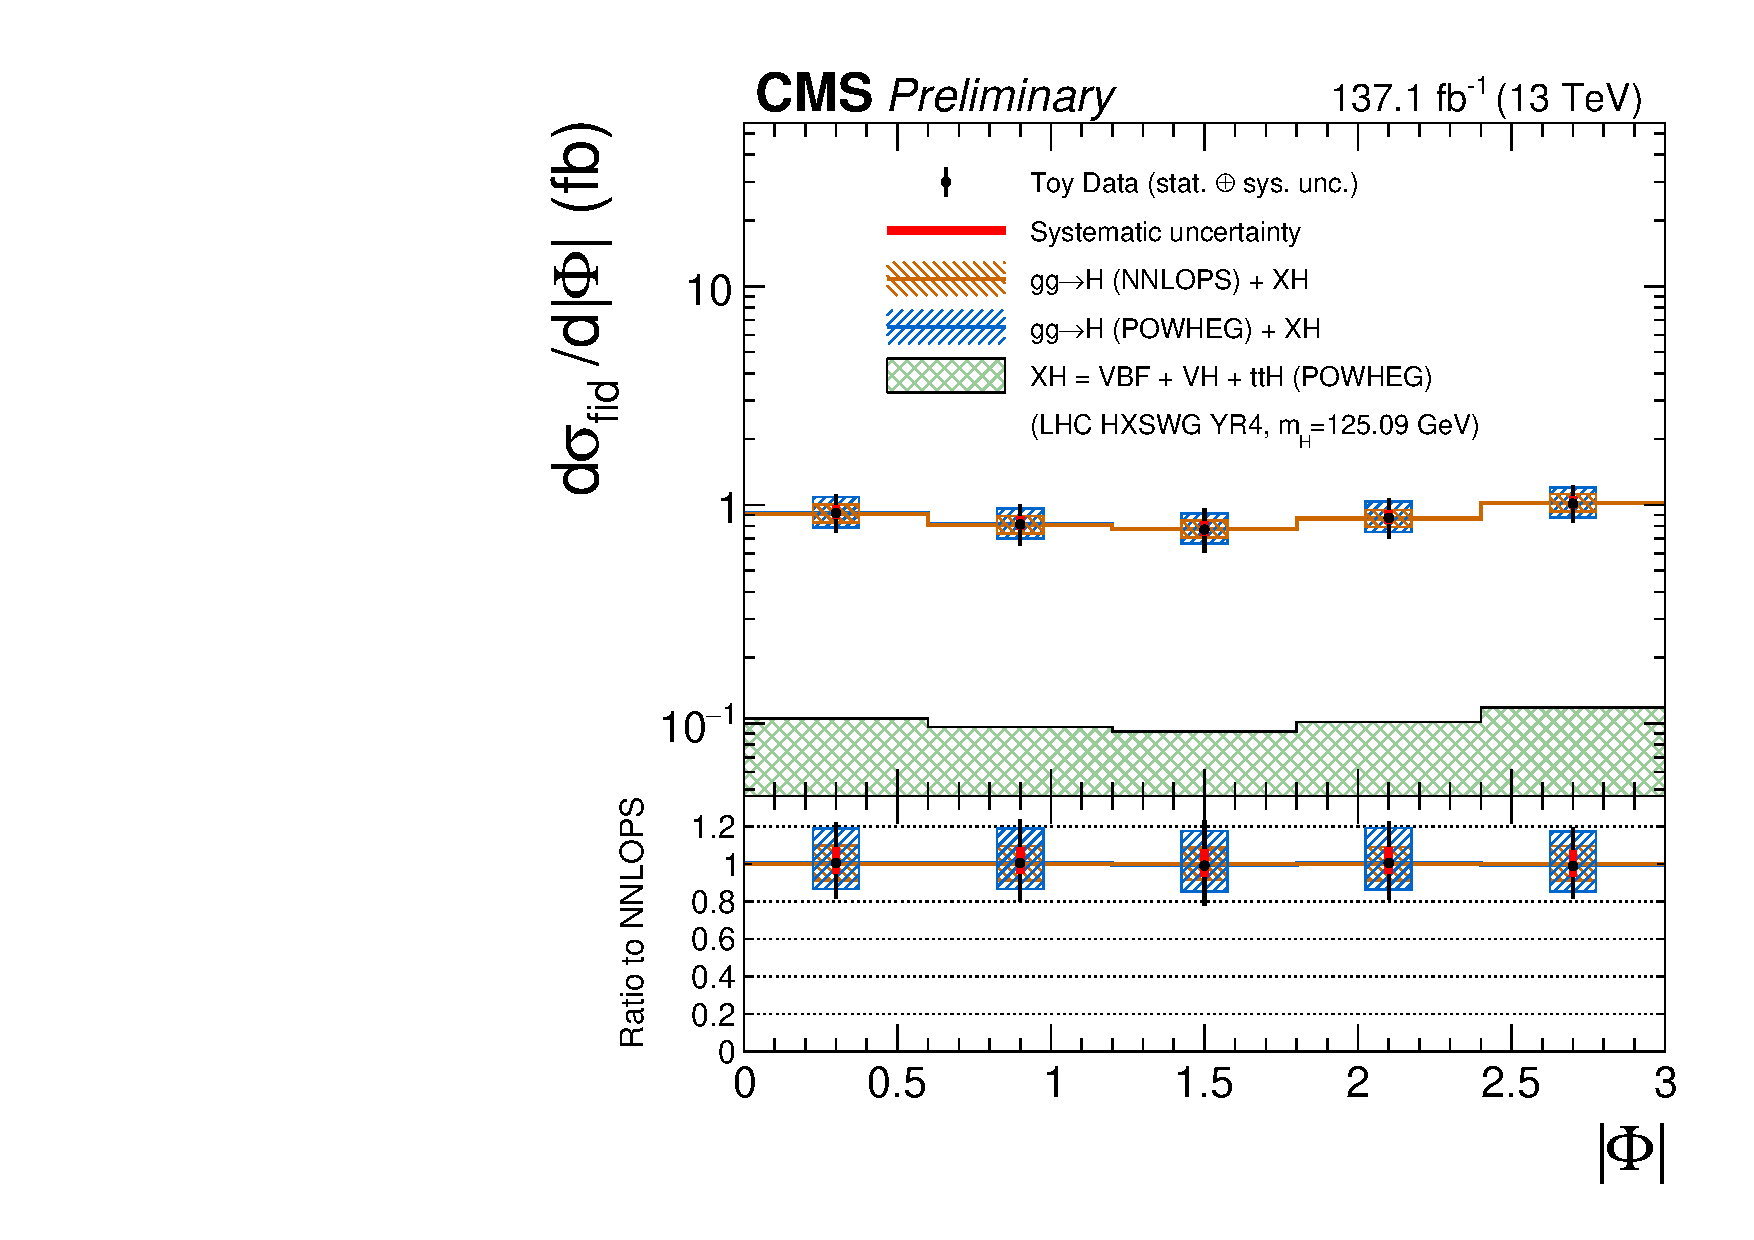
\includegraphics[width=0.45\textwidth,angle=0]{Figures/results/fiducial/2018/Phi_unfoldwith_SM_125_logscale_asimov.pdf}
%      \label{fig:differential-results-ZHasimov:a}
%    }
%	 \subfigure[$\Phi_{1}$]{
%      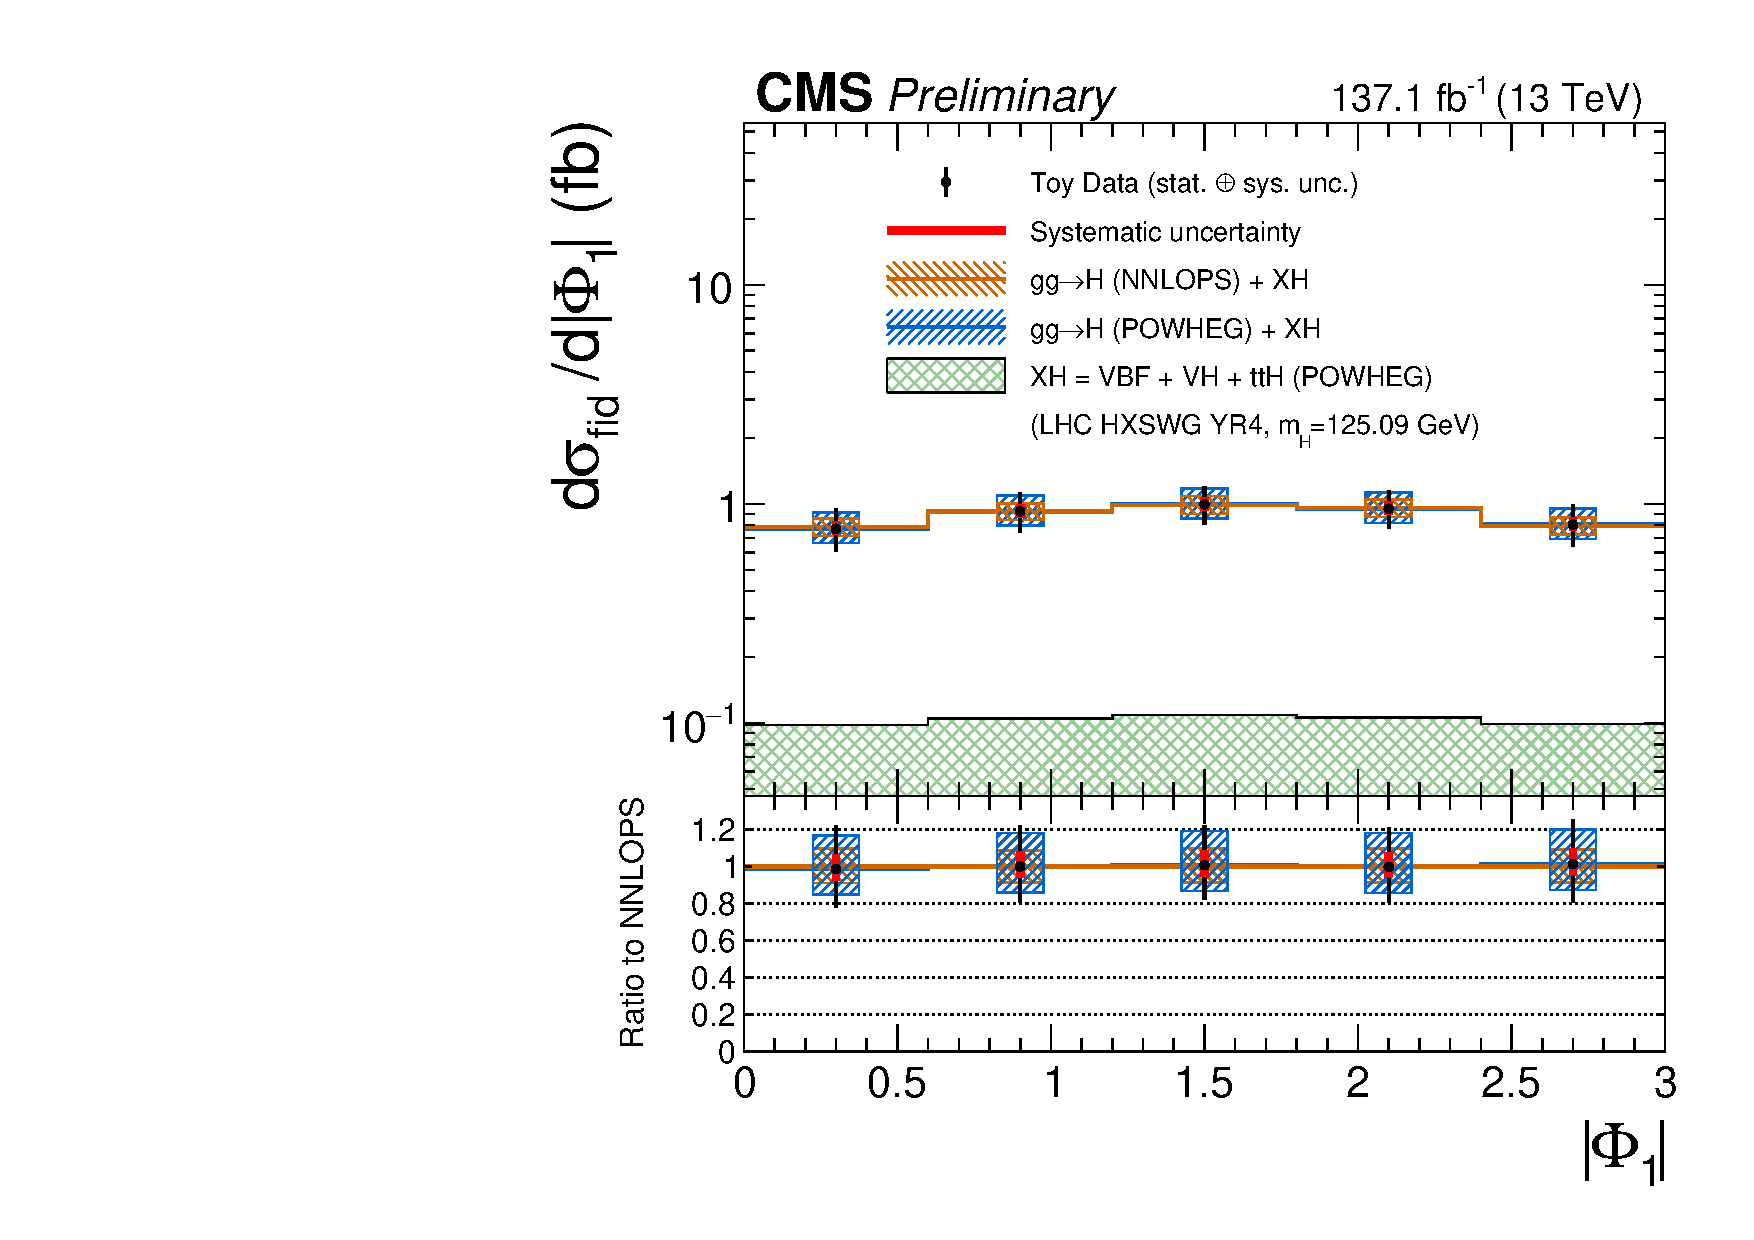
\includegraphics[width=0.45\textwidth,angle=0]{Figures/results/fiducial/2018/Phi1_unfoldwith_SM_125_logscale_asimov.pdf}
%      \label{fig:differential-results-ZHasimov:b}
%    } \\
%	  \subfigure[$\mathrm{m}(\mathrm{Z}_{2})$]{
%      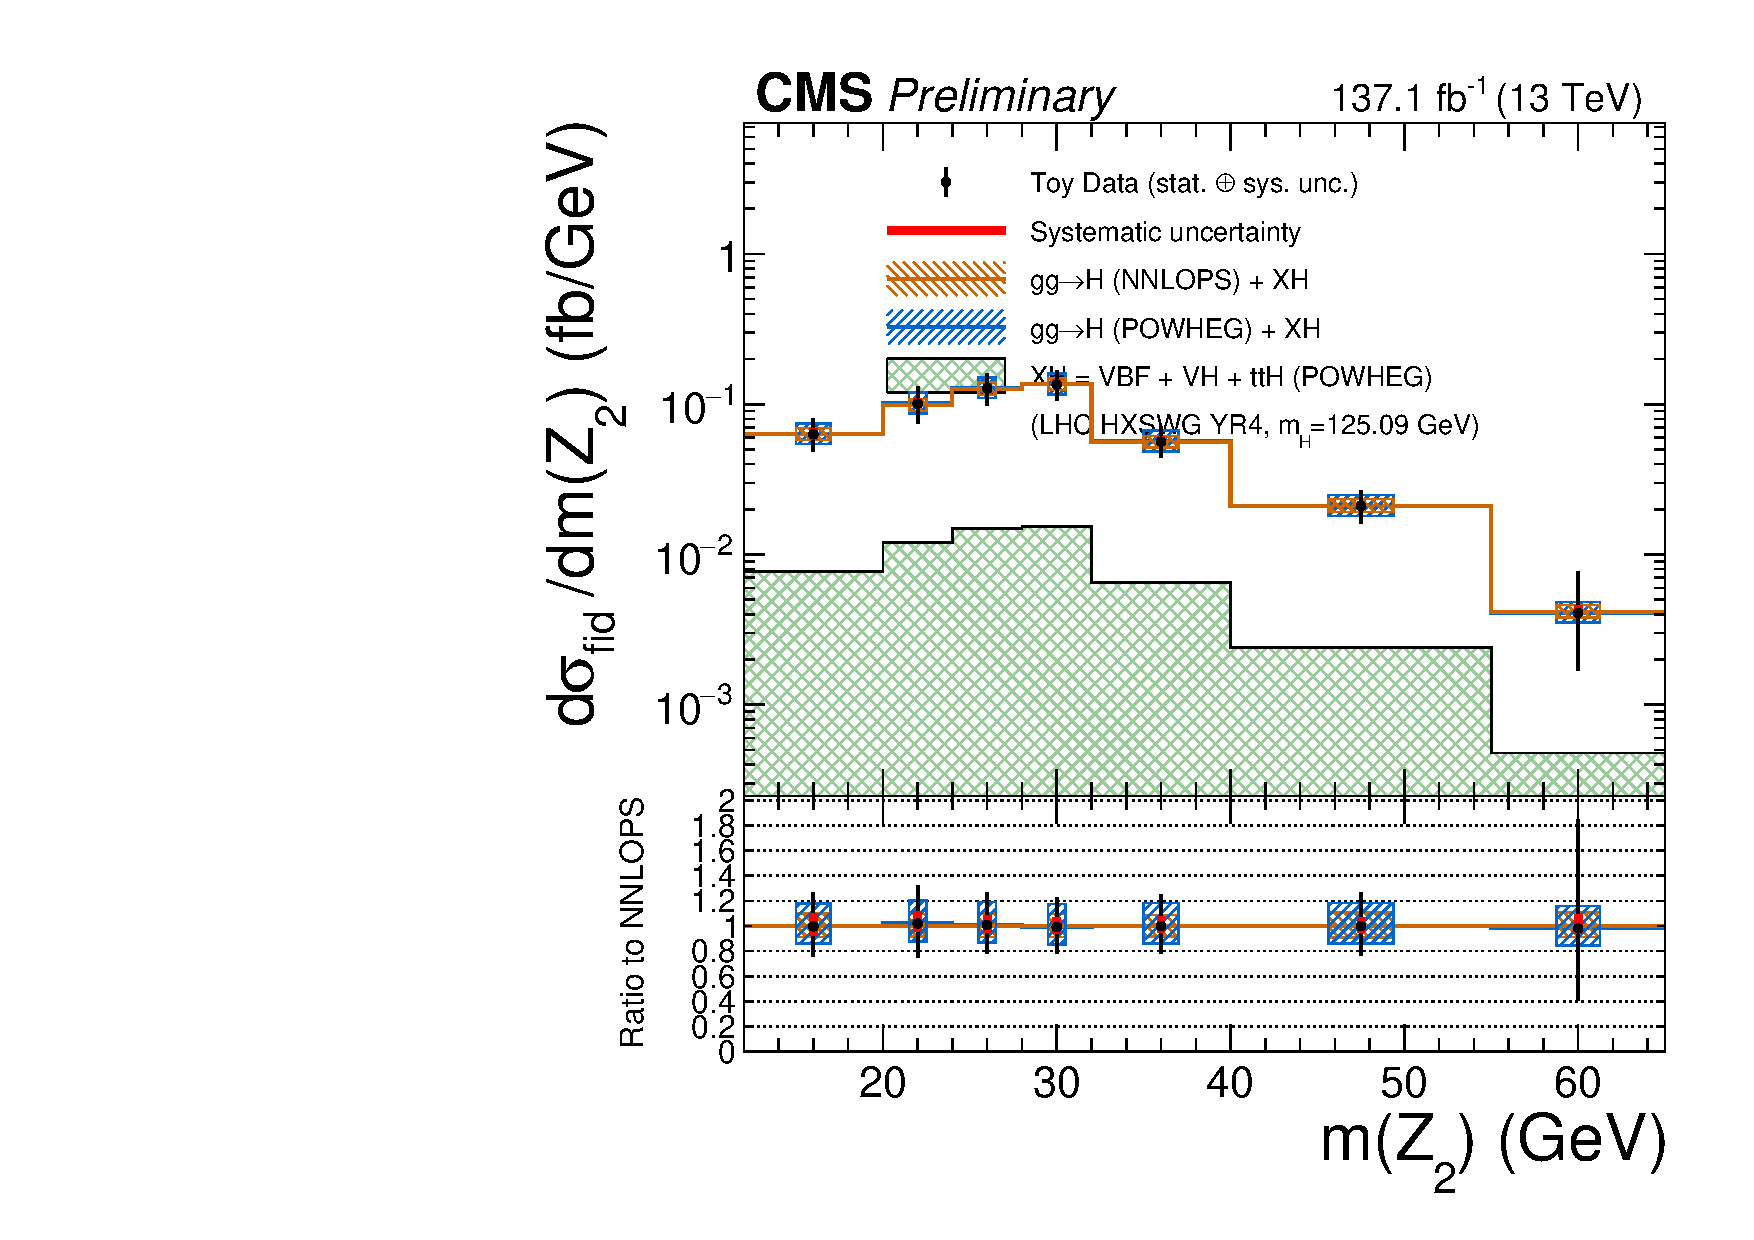
\includegraphics[width=0.45\textwidth,angle=0]{Figures/results/fiducial/2018/massZ2_unfoldwith_SM_125_logscale_asimov.pdf}
%      \label{fig:differential-results-ZHasimov:c}
%    } 
%	\subfigure[$\mathrm{m}(\mathrm{Z}_{1})$]{
%      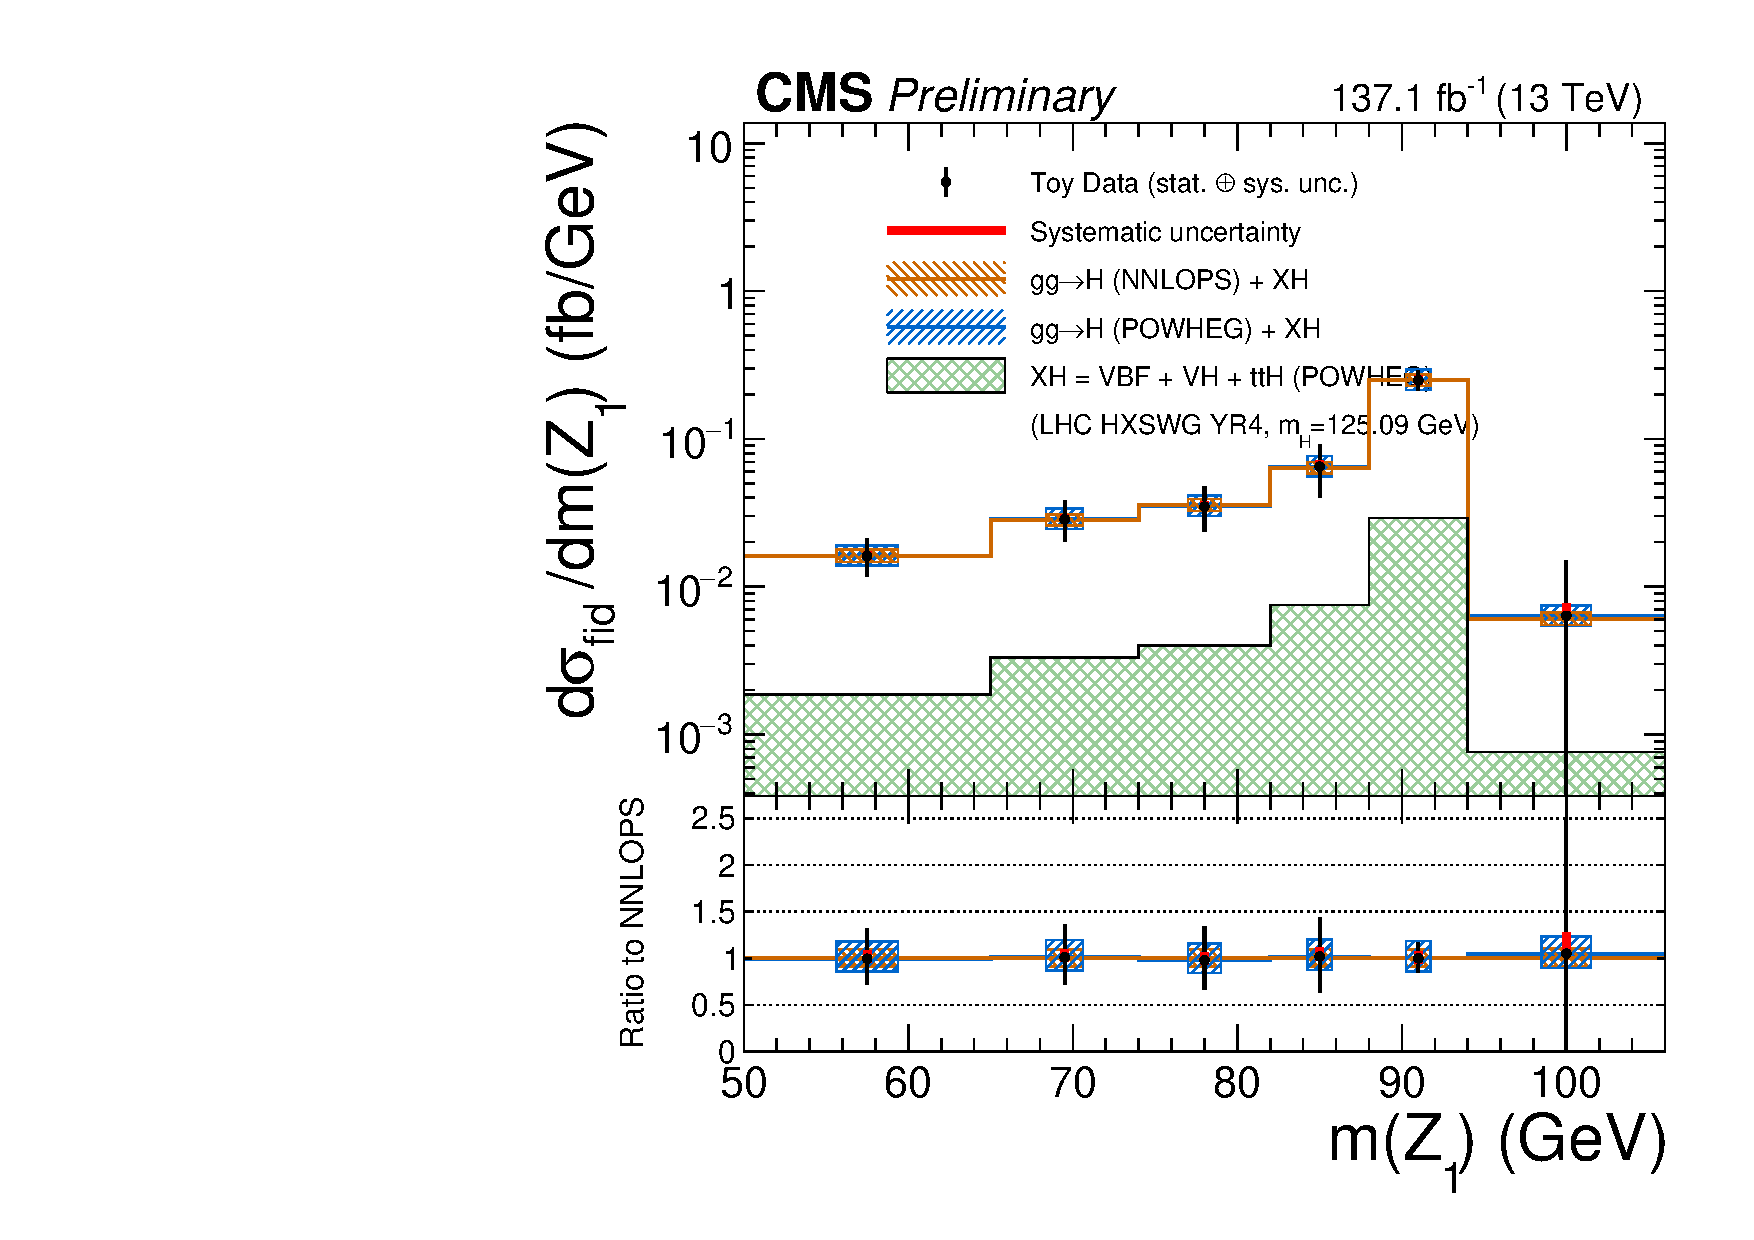
\includegraphics[width=0.45\textwidth,angle=0]{Figures/results/fiducial/2018/massZ1_unfoldwith_SM_125_logscale_asimov.pdf}
%      \label{fig:differential-results-ZHasimov:d}
%    }\\
%    \subfigure[$|\cos \theta^{*}|$]{
%      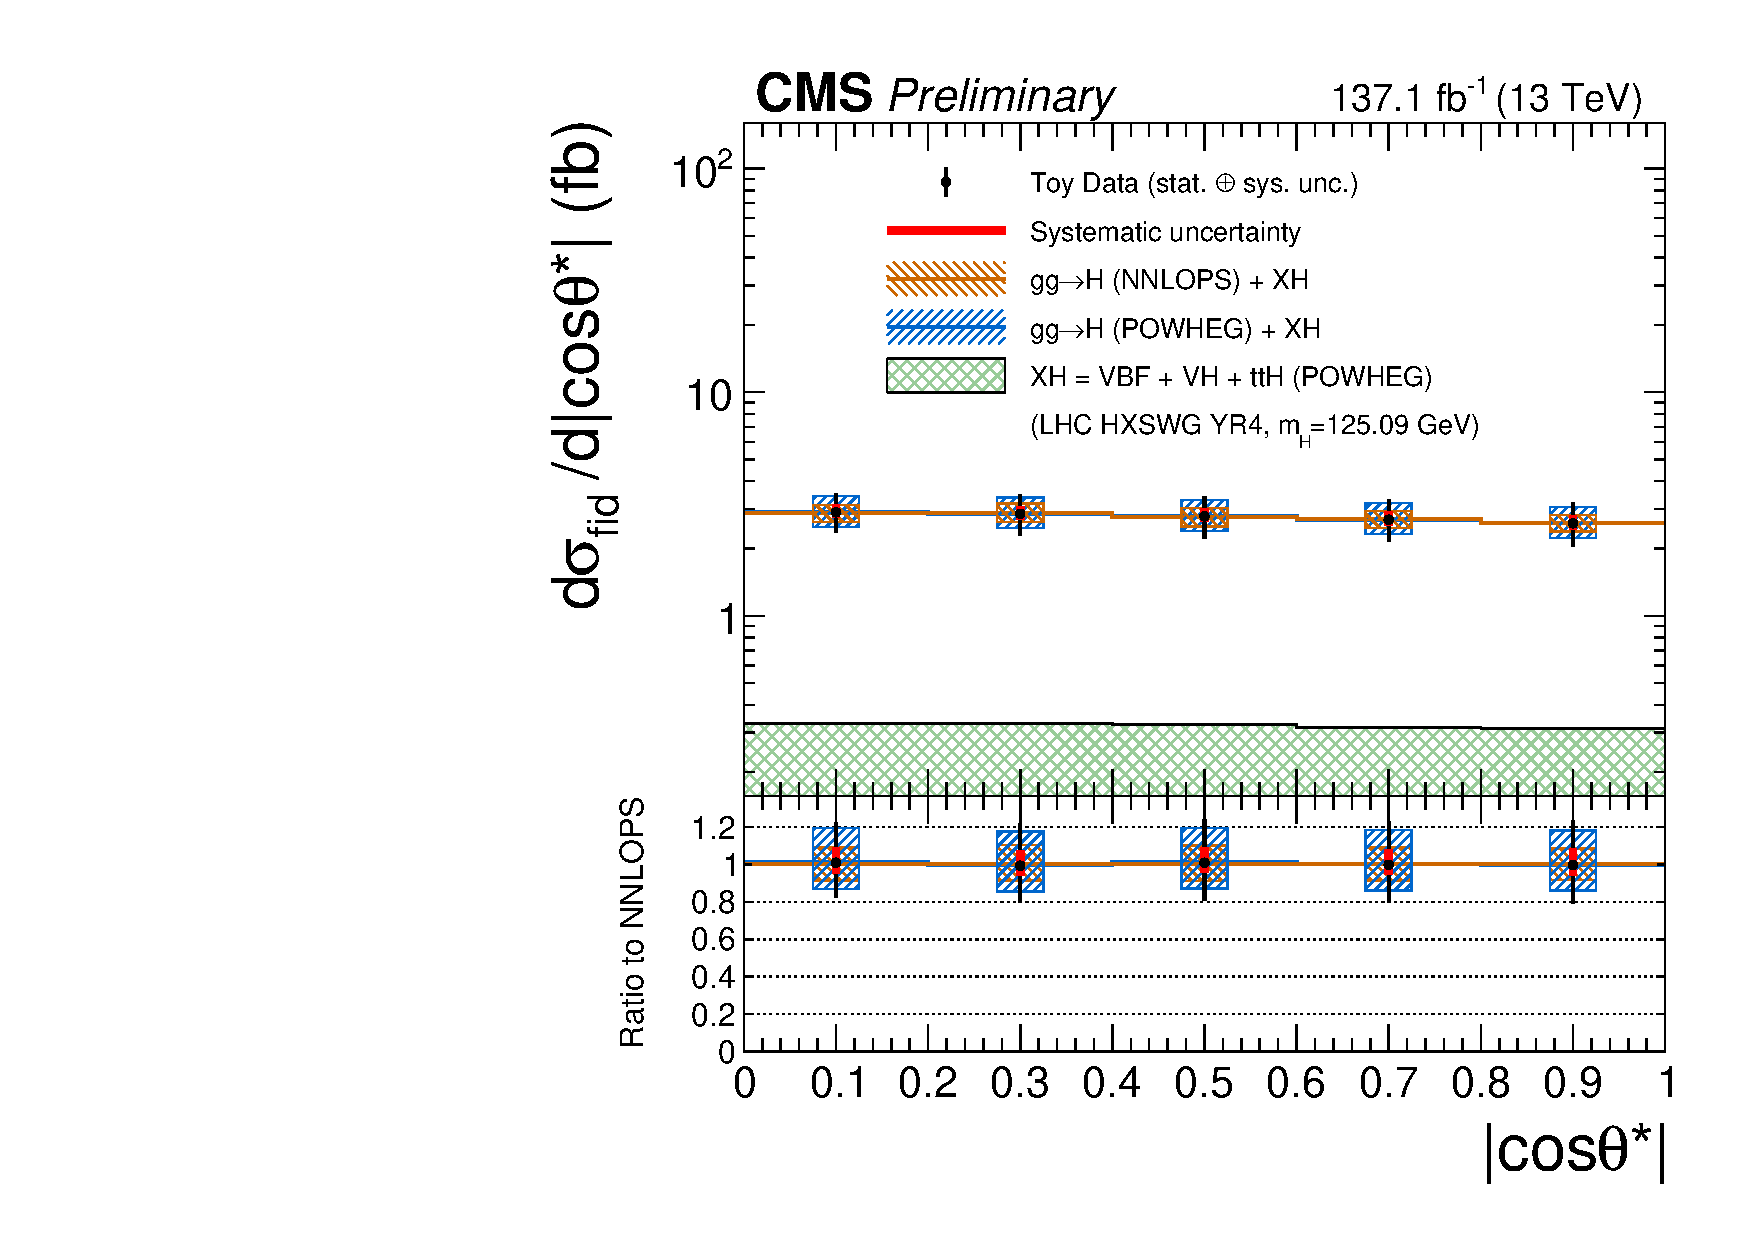
\includegraphics[width=0.45\textwidth,angle=0]{Figures/results/fiducial/2018/cosThetaStar_unfoldwith_SM_125_logscale_asimov.pdf}
%      \label{fig:differential-results-ZHasimov:e}
%    } 
%    \caption{Differential fiducial cross section results using full Run 2 toy data for $\Phi$, $\Phi_{1}$, $\mathrm{m}(\mathrm{Z}_{1})$, $\mathrm{m}(\mathrm{Z}_{2})$ and $|\cos \theta^{*}|$ in $\Hllll$ and comparison with the theoretical predictions. 
%%        Systematic uncertainty is indicated by red bars and black bars show total statistical and the systematic uncertainties, combined in quadrature. The blue and brown colors show the theoretical predictions. 
%%          The acceptances and the theoretical uncertainties in differential bins are computed using {\sc powheg}. Sub-dominant production contributions XH $=$ VBF $+$ VH $+$ $\ttH$ are shown in green separately. The systematic uncertainties correspond to the generators accuracy are also taken in to account for differential predictions. The fraction of $4\mu$, $4e$ and $2e2\mu$ in each differential bin is allowed to float in fit.
%  }
%  \label{fig:differential-results-restrictive_md1}
% \end{center}
%\end{figure} \clearpage
%
%
%
%\begin{figure}[!h!tb]
%  \begin{center}
%          \subfigure[$|\cos \theta_{1}|$]{
%      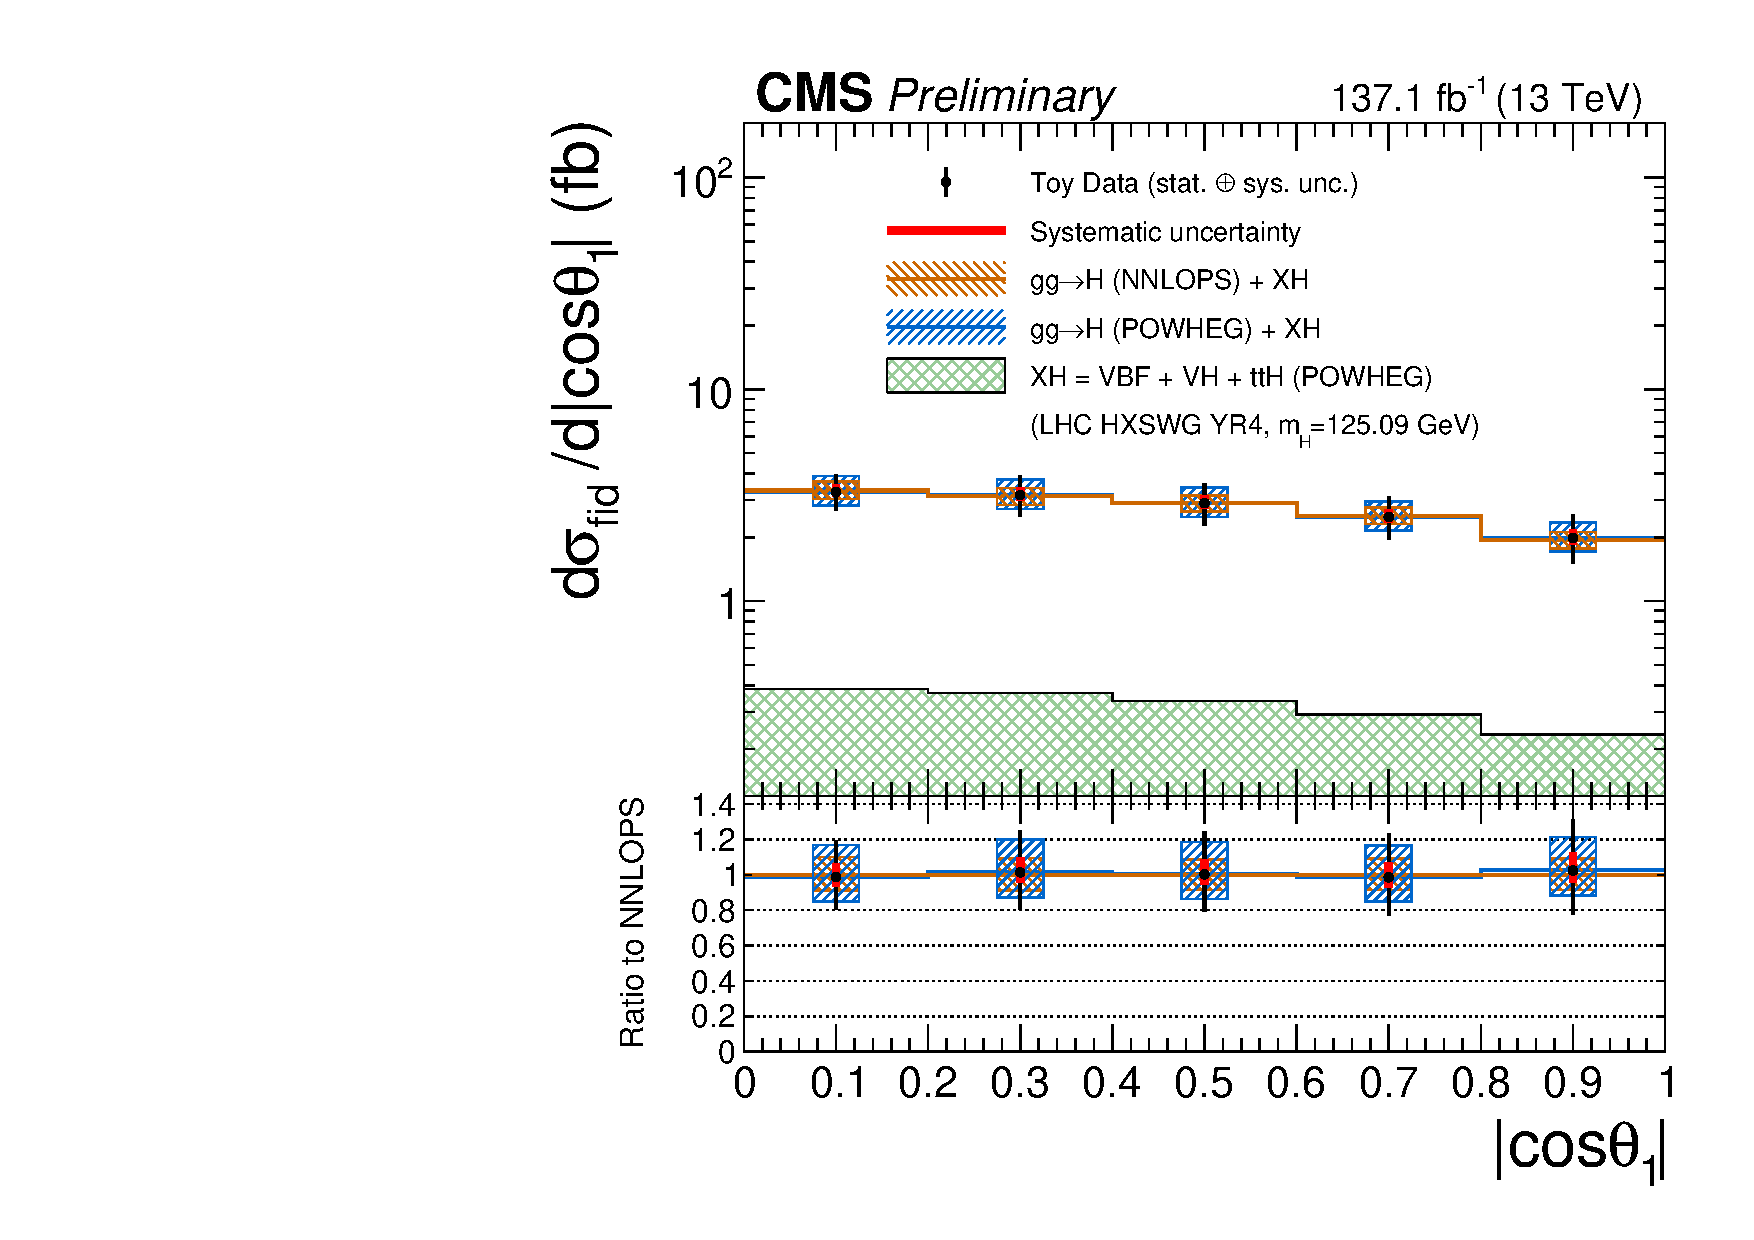
\includegraphics[width=0.45\textwidth,angle=0]{Figures/results/fiducial/2018/cosTheta1_unfoldwith_SM_125_logscale_asimov.pdf}
%      \label{fig:differential-results-ZHasimov1:a}
%    }
%         \subfigure[$|\cos \theta_{2}|$]{
%      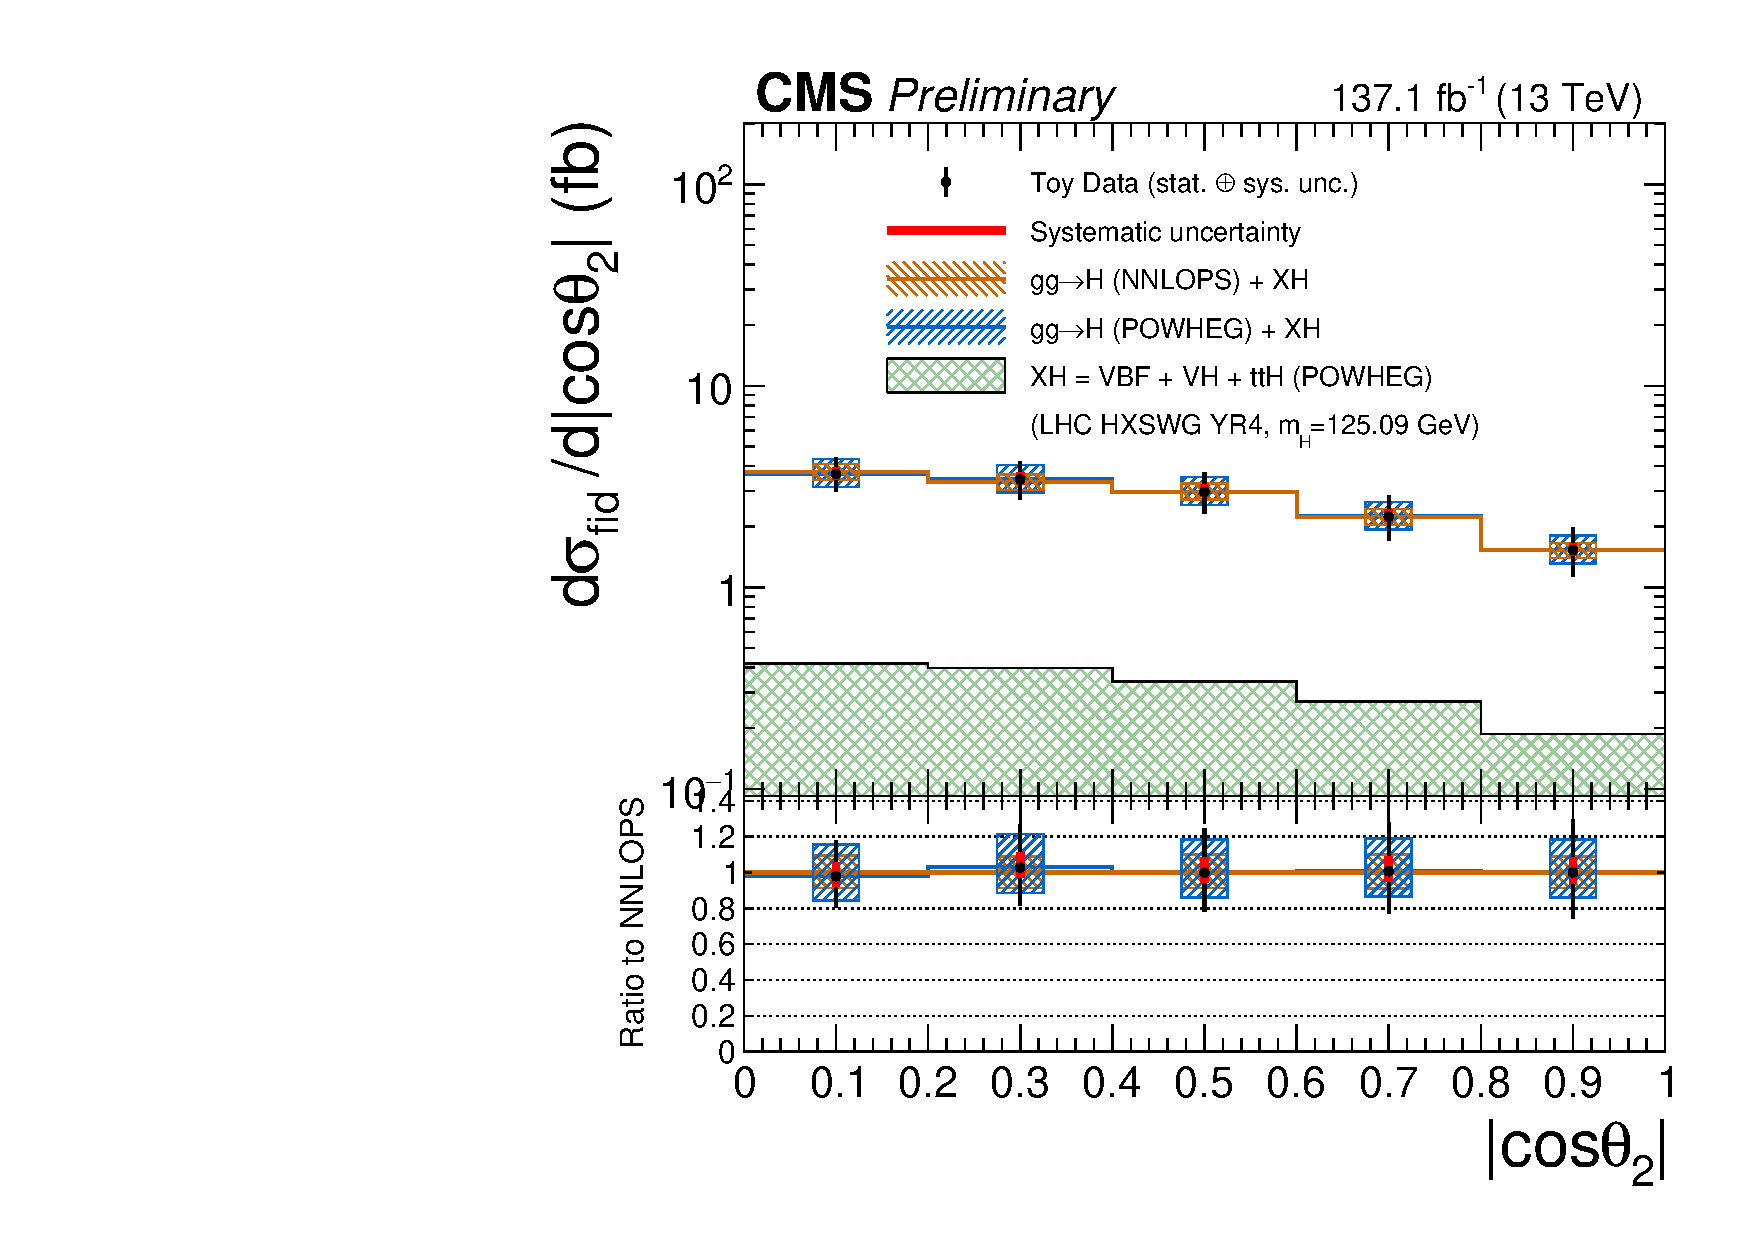
\includegraphics[width=0.45\textwidth,angle=0]{Figures/results/fiducial/2018/cosTheta2_unfoldwith_SM_125_logscale_asimov.pdf}
%      \label{fig:differential-results-ZHasimov1:b}
%    } \\
%%          \subfigure[N(jets) with $|\eta|<4.7$]{
%%      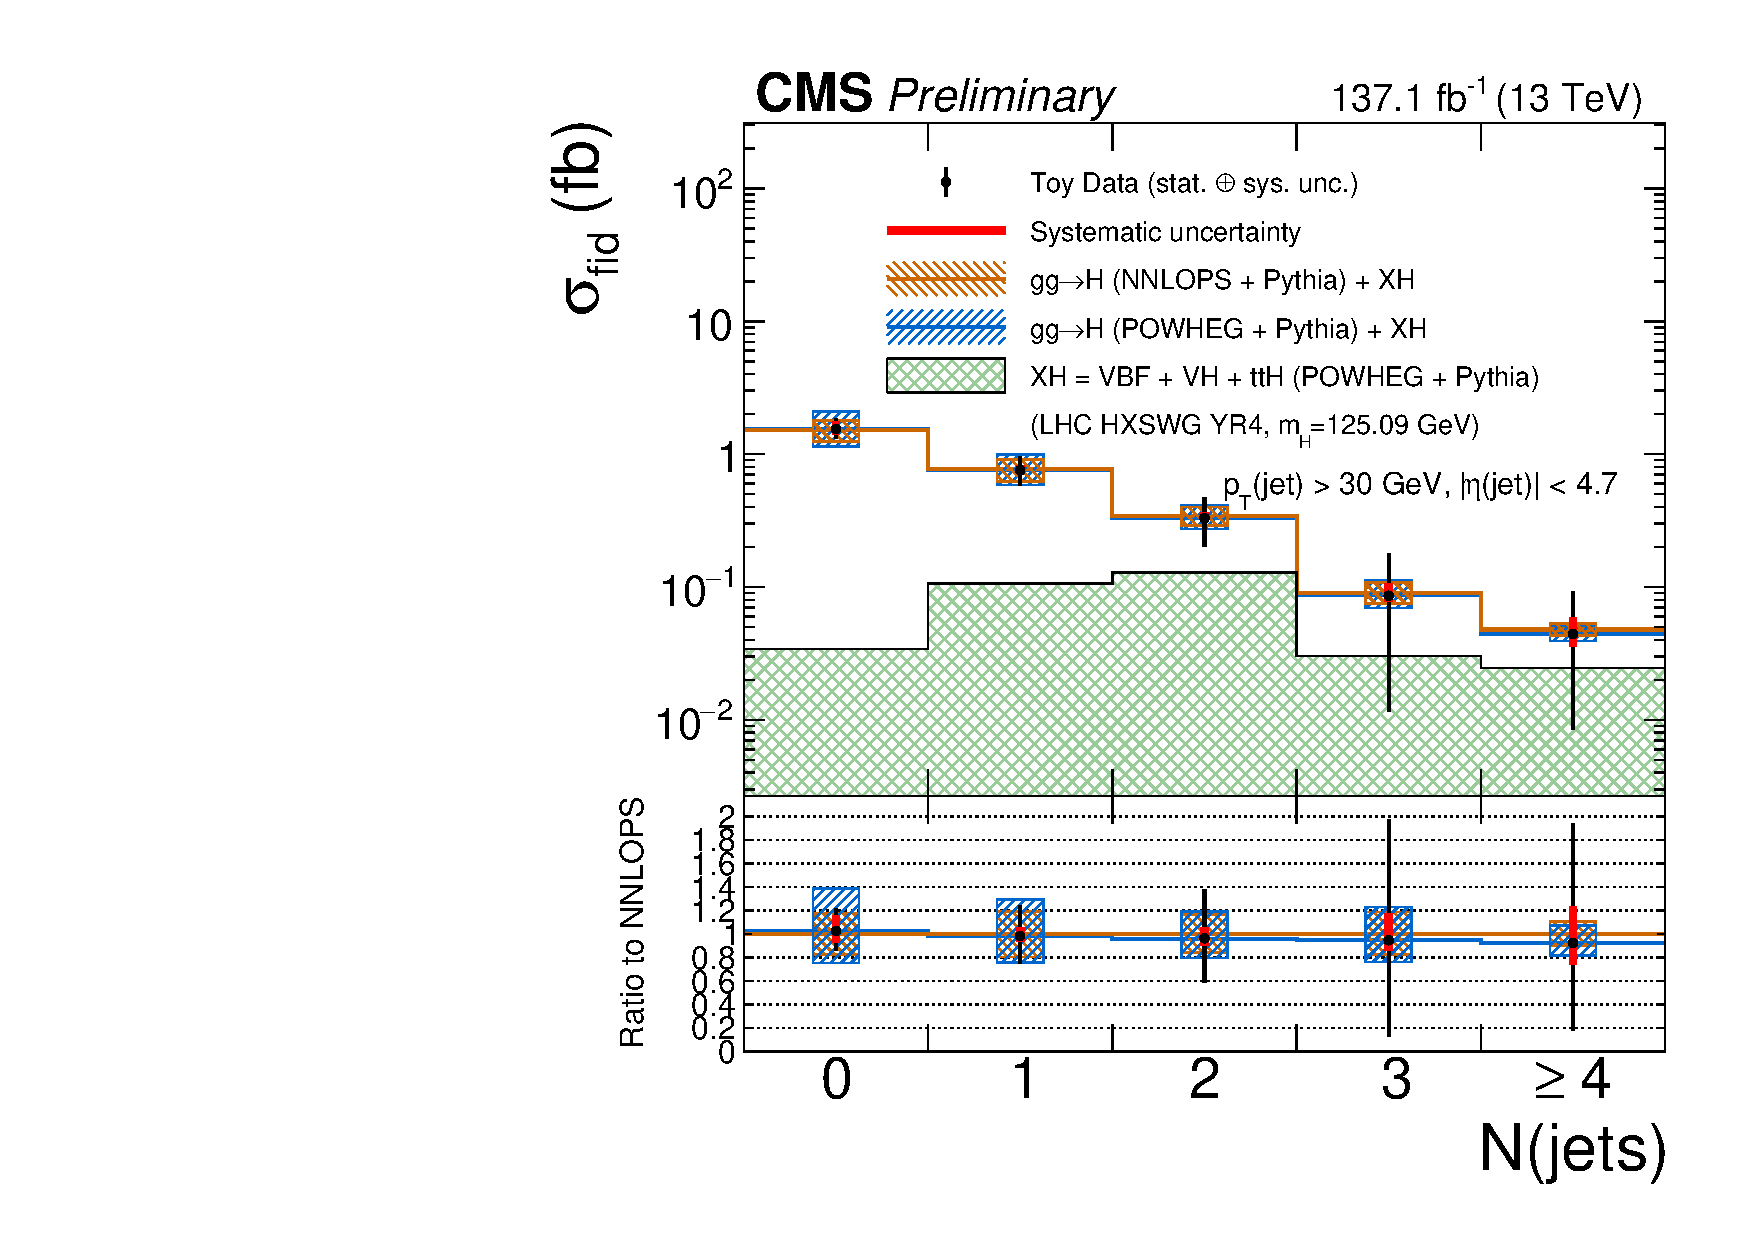
\includegraphics[width=0.45\textwidth,angle=0]{Figures/results/fiducial/2018/njets_pt30_eta4p7_unfoldwith_SM_125_logscale_asimov.pdf}
%%      \label{fig:differential-results-ZHasimov1:c}
%%    }
%%        \subfigure[\pt of leading jet with $|\eta|<4.7$]{
%%      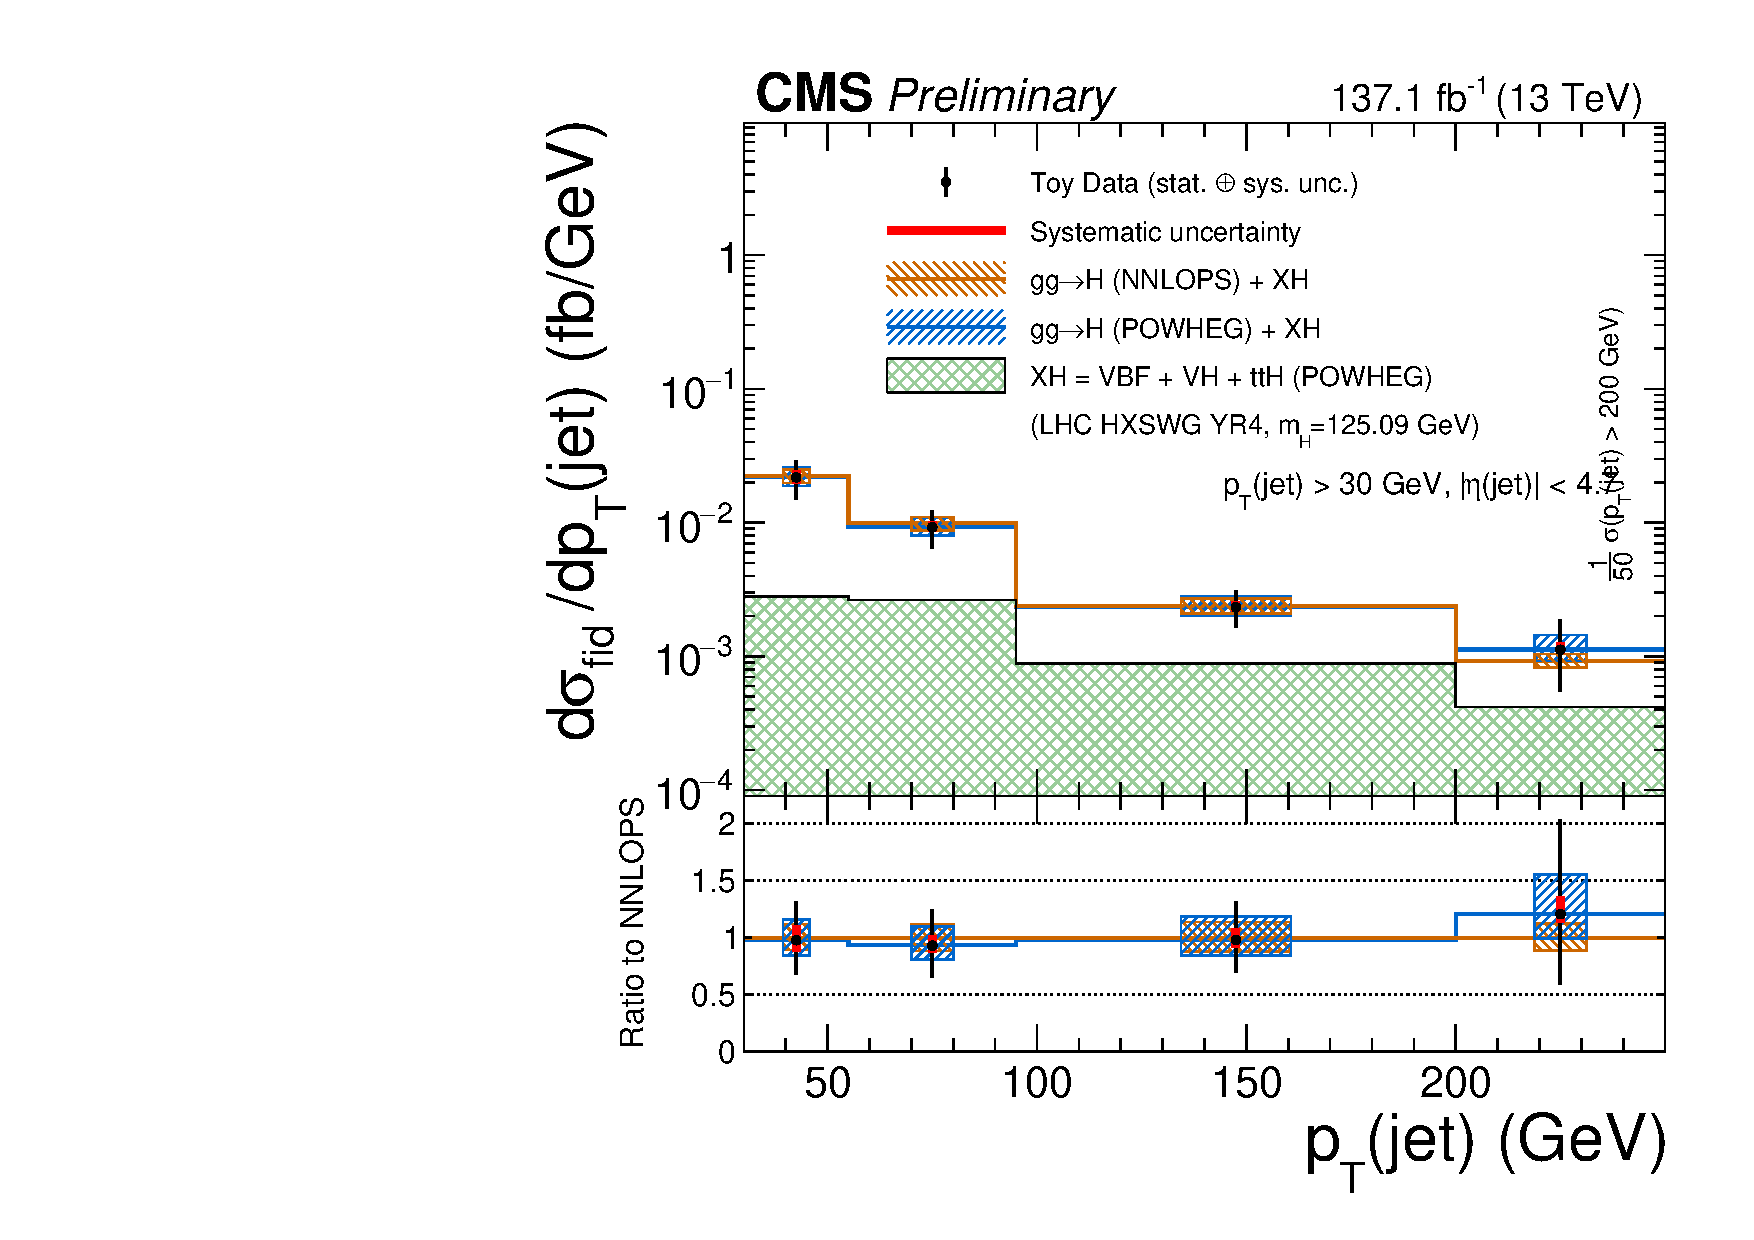
\includegraphics[width=0.45\textwidth,angle=0]{Figures/results/fiducial/2018/pt_leadingjet_pt30_eta4p7_unfoldwith_SM_125_logscale_asimov.pdf}
%%      \label{fig:differential-results-ZHasimov1:d}
%%    }\\
%    \caption{
%	    %Differential fiducial cross section results using full Run 2 toy data for $|\cos \theta_{1}|$, $|\cos \theta_{2}|$, number of jets (within $|\eta|<4.7$) and $\pt$ of leading jet (within $|\eta|<4.7$) in $\Hllll$ and comparison with the theoretical predictions.                          
%	    Differential fiducial cross section results using full Run 2 toy data for $|\cos \theta_{1}|$, $|\cos \theta_{2}|$ in $\Hllll$ and comparison with the theoretical predictions. Systematic uncertainty is indicated by red bars and black bars show total statistical and the systematic uncertainties, combined in quadrature. The blue and brown colors show the theoretical predictions. 
%          The acceptances and the theoretical uncertainties in differential bins are computed using {\sc powheg}. Sub-dominant production contributions XH $=$ VBF $+$ VH $+$ $\ttH$ are shown in green separately. The systematic uncertainties correspond to the generators accuracy are also taken in to account for differential predictions. The fraction of $4\mu$, $4e$ and $2e2\mu$ in each differential bin is allowed to float in fit.                         
%    }
%  \label{fig:differential-results-restrictive_md1}
% \end{center}
%\end{figure} \clearpage
